%%%%%%%%%%%%%%%%%%%%%%%%%%%%%%%%%%%%%%%%%
% Beamer Presentation
% LaTeX Template
% Version 1.0 (10/11/12)
%
% This template has been downloaded from:
% http://www.LaTeXTemplates.com
%
% License:
% CC BY-NC-SA 3.0 (http://creativecommons.org/licenses/by-nc-sa/3.0/)
%
%%%%%%%%%%%%%%%%%%%%%%%%%%%%%%%%%%%%%%%%%

%----------------------------------------------------------------------------------------
%	PACKAGES AND THEMES
%----------------------------------------------------------------------------------------

\documentclass{beamer}

\mode<presentation> {

% The Beamer class comes with a number of default slide themes
% which change the colors and layouts of slides. Below this is a list
% of all the themes, uncomment each in turn to see what they look like.

%\usetheme{default}
%\usetheme{AnnArbor}
%\usetheme{Antibes}
%\usetheme{Bergen}
%\usetheme{Berkeley}
%\usetheme{Berlin}
%\usetheme{Boadilla}
%\usetheme{CambridgeUS}
%\usetheme{Copenhagen}
%\usetheme{Darmstadt}
%\usetheme{Dresden}
%\usetheme{Frankfurt}
%\usetheme{Goettingen}
%\usetheme{Hannover}
%\usetheme{Ilmenau}
%\usetheme{JuanLesPins}
%\usetheme{Luebeck}
\usetheme{Madrid}
%\usetheme{Malmoe}
%\usetheme{Marburg}
%\usetheme{Montpellier}
%\usetheme{PaloAlto}
%\usetheme{Pittsburgh}
%\usetheme{Rochester}
%\usetheme{Singapore}
%\usetheme{Szeged}
%\usetheme{Warsaw}

% As well as themes, the Beamer class has a number of color themes
% for any slide theme. Uncomment each of these in turn to see how it
% changes the colors of your current slide theme.

%\usecolortheme{albatross}
%\usecolortheme{beaver}
%\usecolortheme{beetle}
%\usecolortheme{crane}
\usecolortheme{dolphin}
%\usecolortheme{dove}
%\usecolortheme{fly}
%\usecolortheme{lily}
%\usecolortheme{orchid}
%\usecolortheme{rose}
%\usecolortheme{seagull}
%\usecolortheme{seahorse}
%\usecolortheme{whale}
%\usecolortheme{wolverine}

%\setbeamertemplate{footline} % To remove the footer line in all slides uncomment this line
\setbeamertemplate{footline}[page number] % To replace the footer line in all slides with a simple slide count uncomment this line

\setbeamertemplate{navigation symbols}{} % To remove the navigation symbols from the bottom of all slides uncomment this line
\setbeamertemplate{itemize items}[triangle]
}

\usepackage{graphicx} % Allows including images
\usepackage{booktabs} % Allows the use of \toprule, \midrule and \bottomrule in tables

\usepackage{longtable}
\usepackage{multirow}
\usepackage{dcolumn}
\usepackage{bigstrut}
\usepackage{dcolumn}
\newcolumntype{d}[1]{D{.}{.}{#1}}
%\usepackage[group-separator={.}]{siunitx}
\usepackage{xcolor,colortbl}
\definecolor{Gray}{gray}{0.85}
\usepackage{siunitx}
\usepackage{colortbl}
%\usepackage{arydshln}
\usepackage{adjustbox} % to use adjustbox command - change size of the table
\usepackage{breqn}

\usepackage{rotating}
\usepackage{epstopdf}
\usepackage{ragged2e}
\usepackage{bm}
%\usepackage[longnamesfirst,semicolon]{natbib}
%\bibliographystyle{agsm}
%\usepackage[citestyle=authoryear]{biblatex}
%\usepackage[backend=bibtex,style=authoryear, natbib]{biblatex}
\usepackage[backend=biber, style=authoryear, natbib, uniquename=false]{biblatex}
\bibliography{Lit_mod.bib}
\bibliography{Surprise_Lit.bib}

%----------------------------------------------------------------------------------------
%	TITLE PAGE
%----------------------------------------------------------------------------------------

\title[]{ \textbf{Do Short Sellers Exploit Mispricing Smartly?}}  % The short title appears at the bottom of every slide, the full title is only on the title page


\author[Pavel Lesnevski]{Pavel Lesnevski }
\institute[University of Mannheim]{University of Mannheim}

\date{September 13, 2018} % Date, can be changed to a custom date

\begin{document}

\begin{frame}
\titlepage % Print the title page as the first slide
\end{frame}

%\begin{frame}
%\frametitle{Overview} % Table of contents slide, comment this block out to remove it
%\tableofcontents % Throughout your presentation, if you choose to use \section{} and \subsection{} commands, these will automatically be printed on this slide as an overview of your presentation
%\end{frame}

%----------------------------------------------------------------------------------------
%	PRESENTATION SLIDES
%----------------------------------------------------------------------------------------
%============================================================================

\section{Introduction}
\begin{frame}
	\frametitle{Motivation}
	%\framesubtitle{Bullet points}
	
	\begin{itemize}
		\item Controversial evidence on the ability of institutions to exploit mispricing-based anomalies  on the long side. {\scriptsize[Edelen, Ince, and Kadlec (2016), DeVault, Sias, and Starks (2016), Akbas et al. (2015)]}
		\item General profitability of short positions. {\scriptsize[\citet{desai_investigation_2002}, \citet{boehmer_which_2008}, \citet{diether_short-sale_2009}]} 
		\item Less attention is paid to short sellers' ability to exploit anomalies. Existing papers focus on the value and momentum anomalies. {\scriptsize[Dechow et al. (2001), Hanson and Sunderam (2014)]}
		\item I use aggregate short interest data and the mispricing score of Stambaugh, Yu, and Yuan (2015) to fill in the gap.
		\item I contribute to the literature by answering the following questions:
		\begin{itemize}

			\vspace*{0.1cm}
			\item Do short sellers exploit mispricing?
			\item Do they follow sentiment signal?
			\item Do they trade stocks with high limits to arbitrage strategically?
			\item Do they arbitrage mispricing away?
			\item Do short positions confirm predictions of theoretical models? 
		\end{itemize}
	\end{itemize}
\end{frame}
%============================================================================

\begin{frame}
		\frametitle{Related Papers}
	\begin{itemize}
\item Hanson and Sunderam (2014), RFS
	\begin{itemize}
\item Use time-variation in the cross-section of short interest to show that the significant growth of arbitrage capital exploiting momentum and value strategies is significantly related to the decrease in profitability of these strategies.
 	\end{itemize}
\item Hwang and Liu (2014), WP
	\begin{itemize}
\item Find that short sellers shy away from risky and prefer low-volatility, high-return  strategies  that  have  weak  correlations  with  other  strategies.
	\end{itemize}
\item Wu and Zhang (2015), WP
	\begin{itemize}
\item Show that short interest increasingly contains more return predictive information  beyond  anomalies, especially in more recent years.
	\end{itemize} 

 
% \item Other Related Papers: \citet{Akbas2015}, \citet{Jiao2016}, \citet{Drechsler2016}
	\end{itemize} 

\end{frame}
%============================================================================
\section{Data}
\begin{frame}
	\frametitle{Data}
\begin{itemize}
\item Sample period: March 1980 -- December 2013
\item Sample selection:
\begin{itemize}
\item stocks with share code 10 and 11
\item AMEX, NYSE, NASDAQ traded stocks
\item Price greater than USD 1 and market cap greater than the 5th percentile of the NYSE distribution
\end{itemize}
\ \\
\ \\
\item Equity market data on stock level: CRSP
\item Accounting data: Compustat annual file
\item Short interest: Compustat supplementary short interest file
\item Institutional ownership: TR 13F Filings
\item Mispricing score and risk factors: Authors' websites
\item Analyst coverage: IBES
\end{itemize}
\end{frame}
%============================================================================
\begin{frame}
	\frametitle{Data}

	\begin{itemize}
		\item Mispricing measure (MISP) is the arithmetic average of ranking percentile for each of the 11 mispricing-based anomalies. \citep{Stambaugh2015}
		\begin{itemize}
			\item The alpha and the associated t-statistic are much higher for combined strategy compared to individual anomalies.
			\item Investor sentiment drives the dynamics of each of the 11 individual anomalies. \citep{Stambaugh2012a}
			\item Significant cross-sectional stock return predictability around the globe. \citep{Jacobs2016}
			\item Commonly used in the literature.
			\item Mispricing score is an ordinal value, i.e. it shows only that one stock is more or less overpriced than another stock in the cross-section, but does not show whether the mispricing increased or decreased over time. 
		\end{itemize}	
	\end{itemize}
\end{frame}  
%%========================================
%\begin{frame}
%	\frametitle{Descriptive Statistics}
%\begin{table}[htbp]
%  \centering
%  \footnotesize
%	  \resizebox{0.7\textwidth}{!}{
%	% Table generated by Excel2LaTeX from sheet 'summary'
\begin{tabular}{lccccccc}
\hline
\hline
\multicolumn{8}{l}{Panel A: Summary Statistics} \bigstrut\\
\hline
        &         &         & \multicolumn{5}{c}{Percentiles} \bigstrut\\
\cline{4-8}\multicolumn{1}{c}{Variable} & Mean    & SD      & 1st     & 10th    & Median  & 90th    & 99th \bigstrut\\
\hline
$SUSIR$ & 0.334   & 0.403   & -0.718  & -0.159  & 0.348   & 0.800   & 1.555 \bigstrut[t]\\
$SR$    & 0.027   & 0.023   & 0.003   & 0.005   & 0.018   & 0.060   & 0.094 \\
$DTC$   & 5.479   & 2.142   & 1.467   & 2.095   & 5.787   & 7.959   & 10.046 \\
$SR_{IO}$ & 0.058   & 0.024   & 0.023   & 0.032   & 0.050   & 0.091   & 0.129 \\
$MBETA$ & 1.056   & 0.063   & 0.865   & 0.990   & 1.048   & 1.143   & 1.163 \\
$SIZE$  & 3939.353 & 2230.917 & 896.804 & 1153.332 & 3571.290 & 6905.367 & 8159.658 \\
$BM$    & 0.670   & 0.123   & 0.449   & 0.504   & 0.665   & 0.840   & 0.965 \\
$RET\_RV$ & 0.012   & 0.050   & -0.117  & -0.046  & 0.017   & 0.070   & 0.120 \\
$RET\_MOM$ & 0.185   & 0.208   & -0.283  & -0.067  & 0.178   & 0.413   & 0.851 \\
$INV$   & 0.161   & 0.041   & 0.067   & 0.108   & 0.161   & 0.215   & 0.236 \\
$ROA$   & 0.053   & 0.016   & 0.009   & 0.032   & 0.054   & 0.066   & 0.091 \\
$MISP$  & 48.879  & 1.224   & 45.616  & 47.089  & 49.145  & 50.092  & 51.506 \\
$IVOLA$ & 0.019   & 0.004   & 0.014   & 0.015   & 0.018   & 0.024   & 0.032 \\
$HLSPREAD$ & 0.007   & 0.002   & 0.005   & 0.006   & 0.007   & 0.010   & 0.017 \\
$IO$    & 0.514   & 0.149   & 0.268   & 0.303   & 0.488   & 0.730   & 0.761 \bigstrut[b]\\
\hline
\end{tabular}%

%	\label{tab:summary}%
%	}
%\end{table}
%	\end{frame}
%%========================================
%============================================================================	
\begin{frame}
	\frametitle{Methodology}
	\begin{itemize}
		\item Panel regression adopted from \citet{Hanson2014}:
	\end{itemize}
		\begin{equation} \nonumber 
			SR_{i,t} = T_t + S_i+\bm{\beta}^{MISP\prime}  \bm{D}^{MISP}_{it-1} +\bm{\beta}^{BM\prime} \bm{D}^{BM}_{it-1}+\bm{\beta}^{Size\prime}  \bm{D}^{Size}_{it-1}  +\bm{\gamma}^\prime \bm{x}_{it-1} + \varepsilon_{i,t}
		\end{equation}

\begin{itemize}
\item[]
\begin{itemize}
	\item $T_t$ - month fixed effects
	\item $S_i$ - stock fixed effects
	\item $\bm{D}^{MISP}_{it}$ - vector of mispricing decile dummies
	\item $\bm{\beta}^{MISP\prime}_{it}$- vector of coefficients on mispricing dummies
	\item $\bm{x}_{it}$ - set of control variables (trading volume, institutional ownership, illiquidity, ivola, convertible debt dummy, dummies for stock exchanges, analyst coverage)
	\item Dummies for decile 5 are not included in the regression (reference decile)
	\item Decile 10 is the short side of the anomaly (overpriced), and decile 1  is the long side of the anomaly (underpriced)

\end{itemize}
\end{itemize}
\end{frame}  
%============================================================================
%============================================================================	
\begin{frame}
	\frametitle{Short Interest Ratio by Mispricing Decile}
	\begin{figure}[htbp]
		\centering
		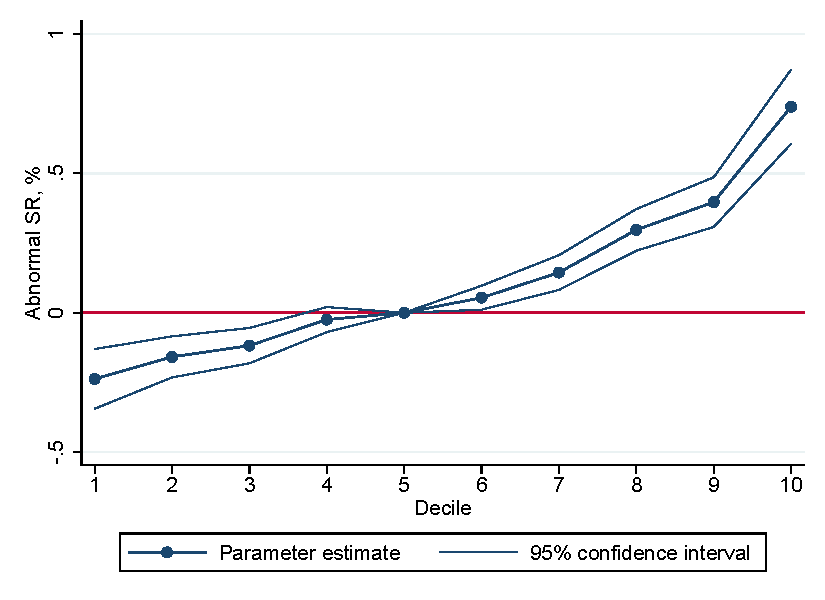
\includegraphics[scale=0.7,trim=4 4 4 4,clip]{figures/misp_sr_by_decile_fe.pdf} 
		\label{tab:misp_evolution_profitability_yq_sentiment}%
	\end{figure}
\vspace*{-0.4cm}
	\begin{itemize}
		\item Strong monotonic relationship between abnormal short interest and mispricing decile.
	\end{itemize}
\end{frame}  
%============================================================================
%%============================================================================
%
%\begin{frame}
%\frametitle{Other variables}
%
%\vspace*{-0.1cm}
%\begin{table}[htbp]
%  \centering
%  \footnotesize
%  	  \resizebox{0.4\textwidth}{!}{	 	
%	 	% Table generated by Excel2LaTeX from sheet 'sr_by_decile_short'
\begin{tabular}{llc}
\toprule
        & \multicolumn{1}{c}{(1)} & (2) \\
        & \multicolumn{1}{c}{SR} & SR \\
\midrule
$Turn$  & \multicolumn{1}{c}{13.29***} & 11.25*** \\
        & \multicolumn{1}{c}{(11.82)} & (12.40) \\
$IO$    & \multicolumn{1}{c}{3.059***} & 6.242*** \\
        & \multicolumn{1}{c}{(12.11)} & (18.10) \\
$IVOL$  & \multicolumn{1}{c}{-2.219} & -2.458 \\
        & \multicolumn{1}{c}{(-0.46)} & (-0.95) \\
$D\_convert$ & \multicolumn{1}{c}{0.641***} & 0.758*** \\
        & \multicolumn{1}{c}{(7.55)} & (9.52) \\
$D\_sp500$ & \multicolumn{1}{c}{-0.463***} & -0.520*** \\
        & \multicolumn{1}{c}{(-5.21)} & (-4.19) \\
$D\_nasdaq$ & \multicolumn{1}{c}{0.920***} & 0.490 \\
        & \multicolumn{1}{c}{(6.11)} & (1.37) \\
$D\_nyse$ & \multicolumn{1}{c}{0.365***} & 0.362** \\
        & \multicolumn{1}{c}{(3.12)} & (2.08) \\
$Illiq$ & \multicolumn{1}{c}{-0.0615**} & -0.0321* \\
        & \multicolumn{1}{c}{(-2.11)} & (-1.86) \\
$Acoverage$ & \multicolumn{1}{c}{0.0305***} & 0.0449*** \\
        & \multicolumn{1}{c}{(4.12)} & (7.76) \\
\midrule
Misp Decile Dummies & \multicolumn{1}{c}{Yes} & Yes \\
SIZE Decile Dummies & \multicolumn{1}{c}{Yes} & Yes \\
BM Decile Dummies & \multicolumn{1}{c}{Yes} & Yes \\
Time Fixed Effects & \multicolumn{1}{c}{Yes} & Yes \\
Stock Fixed Effects & \multicolumn{1}{c}{No} & Yes \\
N       & 575371  & 575279 \\
R-sq    & 0.503   & 0.705 \\
\bottomrule
\end{tabular}%

%	\label{tab:sr_by_decile_short}%
%	}
%\end{table}
%
%\begin{itemize}
%\item[$\rightarrow$] Stock fixed effect account for around 20\% of SR variation.
%\end{itemize}
%	\end{frame}
%
%%============================================================================
%%============================================================================	
%\begin{frame}
%	\frametitle{Short Interest and Sentiment Signal}
%		\framesubtitle{Motivation}	
%	\begin{itemize}
%		\item Motivation 
%	\end{itemize}
%
%\begin{figure}[htbp]
%	\centering
%	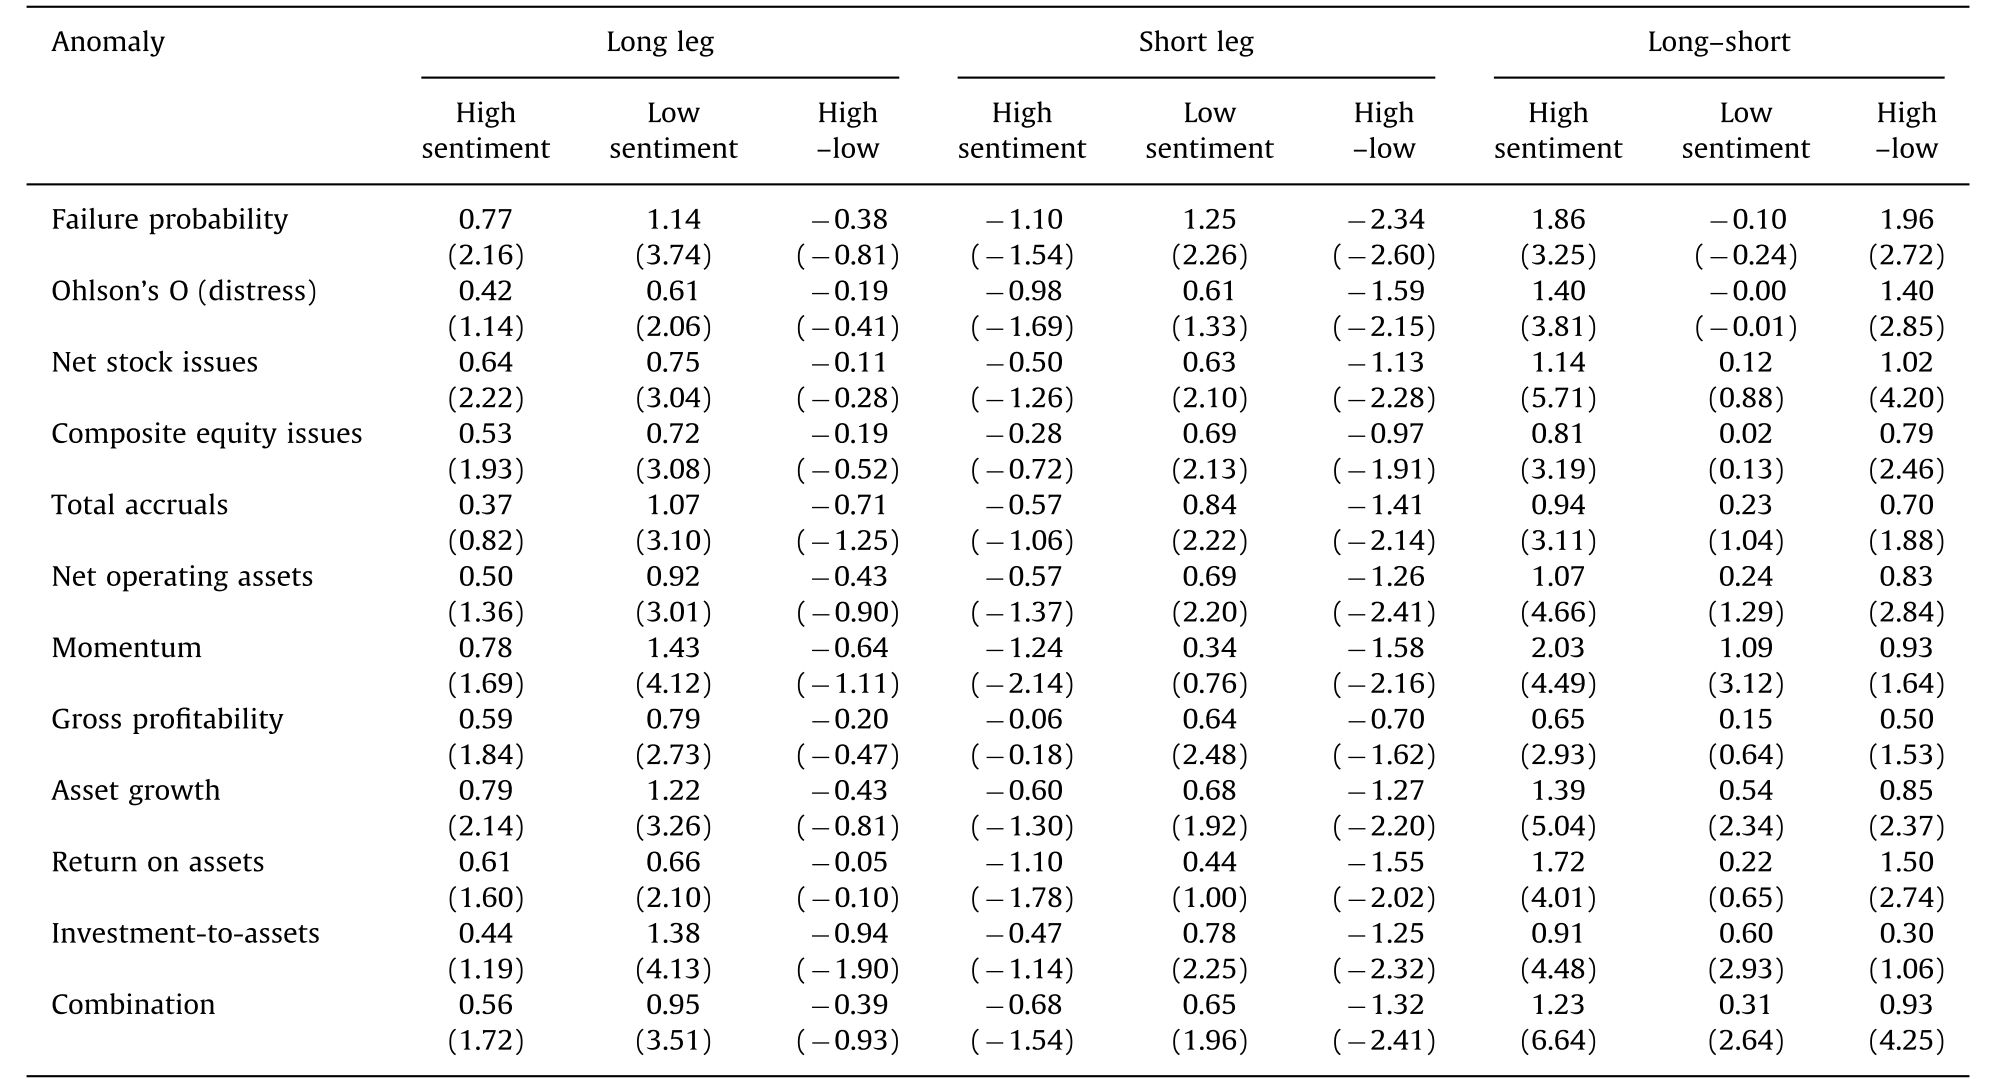
\includegraphics[scale=0.71,trim=0 0 0 0,clip]{figures/motivation_sentiment.jpg} 
%	\label{tab:motivation_sentiment}%
%\end{figure}
%\vspace*{-0.8 cm}
%{\tiny Source: \citet{Stambaugh2012a}}
%\end{frame}  
%============================================================================
%============================================================================	
\begin{frame}
	\frametitle{Short Interest and Sentiment Signal}
		\framesubtitle{Motivation + Methodology}	
	\begin{itemize}
		\item The mispricing anomalies are especially profitable after the periods of high sentiment \citet{Stambaugh2012a}. 
		\item To test whether short sellers react to the change in profitability, I add interaction of sentiment dummy with mispricing decile dummies to the baseline regression:
	\end{itemize}
{\scriptsize
		\begin{equation}		 \nonumber
		\begin{split}
			SR_{i,t} &= Stock_i+\bm{\beta}^{MISP\prime}  \bm{D}^{MISP}_{it-1}+ \bm{\beta}^{HsentD}  HsentD_{t-1} + \bm{\beta}^{MISP \times HsentD\prime}  \bm{D}^{MISP}_{it-1} \times HsentD_{t-1} + \\ 
			&+ \bm{\beta}^{BM\prime}  \bm{D}^{BM}_{it-1}+\bm{\beta}^{Size\prime}_{}  \bm{D}^{Size}_{it-1}  +\bm{\gamma}^\prime \bm{x}_{it-1} + \varepsilon_{i,t}
		\end{split}
		\end{equation}
}
\begin{itemize}
\item[]
\begin{itemize}
	\item $HsentD_{t-1}$ - high sentiment dummy that is equal to 1 if sentiment over the most recent 3 months was above sample median
	\item $\bm{D}^{MISP}_{it} \times HsentD_{t-1}$ - interaction term of mispricing decile dummies with high sentiment dummy

	\item No time fixed effects are included


\end{itemize}
\end{itemize}
\end{frame}  
%============================================================================
%============================================================================
\begin{frame}
		\frametitle{Short Interest and Sentiment Signal}
\vspace*{-.5cm}
		\begin{columns}[t]
 \begin{column}{.32\textwidth} 
 \vspace*{-.45cm} 
\begin{table}[htbp]
  	\resizebox{\textwidth}{!}{
	 	% Table generated by Excel2LaTeX from sheet 'sentiment_misp_short'
\begin{tabular}{lc}
\toprule
      & SR \\
\midrule
$HsentD$ & 0.366*** \\
      & (4.60) \\
$MISP_{Decile = 10} \times HsentD$ & 0.268** \\
      & (2.26) \\
$MISP_{Decile = 9} \times HsentD$ & 0.185** \\
      & (2.31) \\
$MISP_{Decile = 8} \times HsentD$ & 0.189*** \\
      & (2.74) \\
$MISP_{Decile = 7} \times HsentD$ & 0.168*** \\
      & (2.93) \\
$MISP_{Decile = 6} \times HsentD$ & 0.0891** \\
      & (2.22) \\
$MISP_{Decile = 4} \times HsentD$ & -0.0136 \\
      & (-0.32) \\
$MISP_{Decile = 3} \times HsentD$ & -0.0957* \\
      & (-1.87) \\
$MISP_{Decile = 2} \times HsentD$ & -0.164*** \\
      & (-2.81) \\
$MISP_{Decile = 1} \times HsentD$ & -0.271*** \\
      & (-3.91) \\
\midrule
Control Variables & Yes \\
SIZE Decile Dummies & Yes \\
BM Decile Dummies & Yes \\
MISP Decile Dummies & Yes \\
Time Fixed Effects & No \\
Stock Fixed Effects & Yes \\
N     & 575279 \\
R-sq  & 0.687 \\
\bottomrule
\end{tabular}%

	\label{tab:surp}%
	}
\end{table} 
\end{column}
\begin{column}{.68\textwidth}
\begin{itemize}
\item After the period of high sentiment, SR increases for reference stocks by 0.37 p.p.
\item The increase is higher by 0.27 p.p. for the most overpriced stocks, adding up to 0.63 p.p.
\item For the most underpriced stocks, the increase amounts to insignificant 0.1 p.p.
\item[$\Rightarrow$] Arbitrageurs allocate more capital to mispricing strategies after the periods of high sentiment to earn higher abnormal returns. 
\end{itemize}
\end{column}
   \end{columns}
\end{frame}

%============================================================================
%============================================================================
\begin{frame}
\begin{center}
\Large Short Interest and Limits to Arbitrage
\end{center}

\end{frame}
%============================================================================
%============================================================================	
\begin{frame}
	\frametitle{Short Interest and Limits to Arbitrage}
		\framesubtitle{Motivation}
	\begin{itemize}
		\item Higher limits to arbitrage are associated with larger mispricing returns \citep{Stambaugh2015,Chu2016}. 
		\item Do limits to arbitrage stop short sellers from exploiting mispricing?
		\item To answer this question, I analyse the effect of two proxies:
		\begin{itemize}
		\item Idiosyncratic volatility (IVOL), a common proxy for arbitrage risk (\citet{Shleifer1997}; \citet{Pontiff2006}; \citet{Stambaugh2015}; \citet{Drechsler2016}). I use the setting from \citet{Stambaugh2015} to test the relation between IVOL and short positions.
		\item Short sale constraints, proxied by short sale price tests. Regulation SHO serves as a natural experiment to test the effect of these constraints.
		\end{itemize}
	\end{itemize}
\end{frame}  
%============================================================================
%============================================================================	
\begin{frame}
	\frametitle{Short Interest and IVOL}
		\framesubtitle{Motivation}
\begin{figure}[htbp]
\centering
	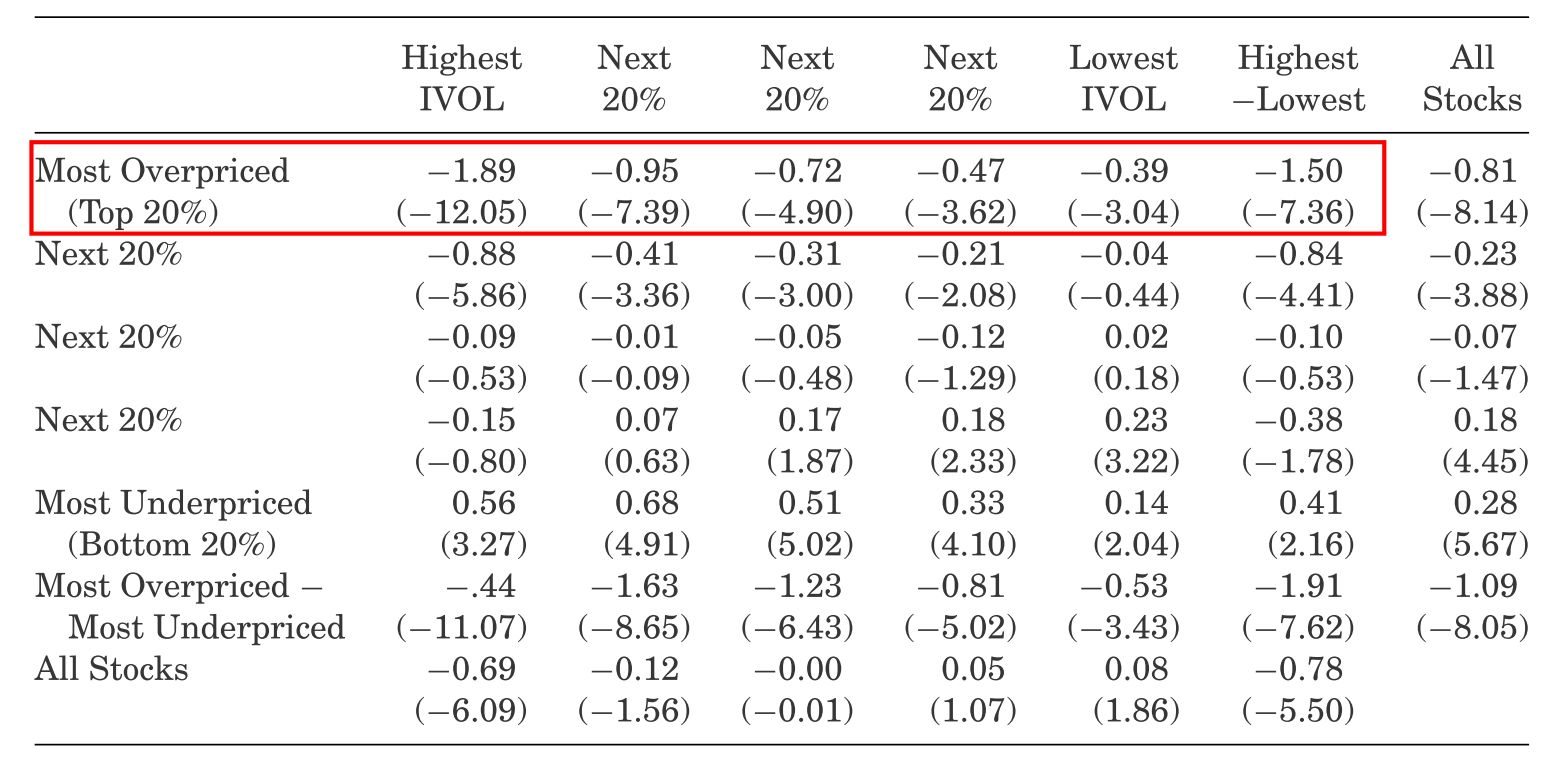
\includegraphics[scale=0.9,trim=1 1 1 1,clip]{figures/motivation_ivol.jpg} 
	\label{tab:SHO_misp_graph}%
\end{figure}
\vspace*{-0.6 cm}
{\tiny \qquad Source: \citet{Stambaugh2015}}
	\begin{itemize}
		\item[$\rightarrow$] Among overpriced stocks, high-IVOL stocks deliver the most negative abnormal returns.  
	\end{itemize}
\end{frame}  
%============================================================================
%===========================================================================

\begin{frame}
	\frametitle{Short Interest and IVOL}
		\framesubtitle{Methodology}	
	\begin{itemize}
		\item To test whether in overpriced stocks IVOL deters or attracts short sellers, I add the interaction of IVOL with mispricing decile dummies to the baseline regression:
	\end{itemize}
{\scriptsize
		\begin{equation}		 \nonumber
		\begin{split}
			SR_{i,t} &= Stock_i+\bm{\beta}^{MISP\prime}  \bm{D}^{MISP}_{it-1}+ \bm{\beta}^{IVOL} IVOL_{t-1} + \bm{\beta}^{MISP \times IVOL\prime}  \bm{D}^{MISP}_{it-1} \times IVOL_{t-1} + \\ 
			&+ \bm{\beta}^{BM\prime}  \bm{D}^{BM}_{it-1}+\bm{\beta}^{Size\prime} \bm{D}^{Size}_{it-1}  +\bm{\gamma}^\prime \bm{x}_{it} + \varepsilon_{i,t}
		\end{split}
		\end{equation}
}
\begin{itemize}
\item[]
\begin{itemize}
	\item $IVOL_{t-1}$ - standard deviation of the most recent month’s daily benchmark-adjusted returns \citep{Stambaugh2015}
	\item $\bm{D}^{IVOL}_{it} \times IVOL{t-1}$ - interaction term of mispricing decile dummies with high sentiment dummy
\end{itemize}
\end{itemize}
\end{frame}  

%============================================================================



%============================================================================
\begin{frame}[label=ivol_results]
		\frametitle{Short Interest and IVOL}

		\begin{columns}[t]
 \begin{column}{.37\textwidth} 
\vspace*{-0.8cm}
\begin{table}[htbp]
  	\resizebox{\textwidth}{!}{
	 	% Table generated by Excel2LaTeX from sheet 'ivola_misp'
\begin{tabular}{lcc}
\toprule
      & (1)   & (2) \\
      & SR    & SR \\
\midrule
$IVOL$ & -6.351* & -5.837* \\
      & (-1.74) & (-1.80) \\
$MISP_{Decile = 10} \times IVOL$ & 18.28*** & 16.44*** \\
      & (3.89) & (4.06) \\
$MISP_{Decile = 9} \times IVOL$ & 10.56** & 10.98*** \\
      & (2.47) & (3.30) \\
$MISP_{Decile = 8} \times IVOL$ & 15.52*** & 10.67*** \\
      & (3.98) & (3.84) \\
$MISP_{Decile = 7} \times IVOL$ & 3.453 & 2.635 \\
      & (1.13) & (1.31) \\
$MISP_{Decile = 6} \times IVOL$ & -0.654 & -0.567 \\
      & (-0.25) & (-0.39) \\
$MISP_{Decile = 4} \times IVOL$ & 0.879 & 2.155 \\
      & (0.34) & (1.43) \\
$MISP_{Decile = 3} \times IVOL$ & 3.503 & 1.071 \\
      & (1.09) & (0.50) \\
$MISP_{Decile = 2} \times IVOL$ & 1.360 & 1.410 \\
      & (0.36) & (0.52) \\
$MISP_{Decile = 1} \times IVOL$ & 2.032 & 2.764 \\
      & (0.46) & (0.76) \\
\midrule
Other Control Variables & Yes   & Yes \\
MISP Decile Dummies & Yes   &  \\
MISP Piecewise Linear &       & Yes \\
Stock Fixed Effects & Yes   & Yes \\
Time Fixed Effects & Yes   & Yes \\
N     & 575279 & 575279 \\
R-sq  & 0.705 & 0.705 \\
\bottomrule
\end{tabular}%

	\label{tab:ivola_misp}%
	}
\end{table} 
\end{column}
\begin{column}{.63\textwidth}
\begin{itemize}
\item One SD increase in IVOL in 5th mispricing decile results in $(0.01* 6.351 * 100)\approx 6$ b.p. decrease in short interest  
\item In contrast, positive SR-IVOL relation for overpriced stocks, one SD increase in IVOL is associated with an increase in SR of 12 b.p.
\item Results are robust to non-linearities in MISP
\item[$\Rightarrow$] Short sellers earn abnormal returns of high-IVOL stocks.
% despite of associated limits to arbitrage. 
\end{itemize}
\hfill \hyperlink{ivol_dynamics}{\beamerbutton{Entering Extreme Deciles}}
\end{column}
   \end{columns}
\end{frame}

%============================================================================

%============================================================================
\begin{frame}
	\frametitle{Short Interest and IVOL}
		\framesubtitle{Discussion}	
\begin{itemize}
\item The observed period follows the period when mispricing builds up. If high IVOL stops arbitrageurs from arbitraging away mispricing at initiation, then high-IVOL stocks are associated higher mispricing in the following period. Smart short-sellers profit from these more mispriced stocks, whose value converges to its fundamental value during the observed period. 

\item These results are broadly consistent with the models of \citet{Stambaugh2015} and \citet{Shleifer1997}.

\item Possible caveats:
 \begin{itemize}
 	\item Lending fees
 	\item Recall risk and other types of short-selling risk 
 \end{itemize}
 
\end{itemize}
\end{frame}  
%============================================================================

%%============================================================================
%\begin{frame}
%	\frametitle{Short Interest and IVOL}
%		\framesubtitle{Discussion}	
%\begin{itemize}
%\item \citet{Stambaugh2015} show empirically that, for a given level of MISP, the returns from shorting overpriced stocks increase with IVOL.
%\item Authors' model predict in equilibrium that, for a given demand shock, short interest of overpriced stocks should not be related to their IVOL. Higher abnormal returns are a compensation for arbitrage risk that attracts arbitrage capital to absorb a given demand shock. 
%\item Alternative models of \citet{Shleifer1997}, \citet{Pontiff2006} and \citet{Drechsler2016} predict negative relation of short positions in overpriced stocks to IVOL for a given level of mispricing. These models imply that IVOL deters arbitrageurs.
%\item[$\Rightarrow$] Long-term short sellers profit from mispricing despite of limits of arbitrage.
% 
%\end{itemize}
%\end{frame}  
%%============================================================================
%%============================================================================
%\begin{frame}
%	\frametitle{Short Interest and IVOL}
%		\framesubtitle{Hypothesis}	
%
%\begin{itemize}
%\item \textbf{Potential resolution of the puzzle:} 
%\begin{itemize}
%\item Stock's demand shock is correlated with IVOL within a given mispricing decile.
%\item Larger mispricing opportunities attract more short sellers.
%\end{itemize}
%\item \textbf{Source of additional mispricing:} Demand shocks to sentiment-prone stocks. IVOL is a key sentiment characteristic in the literature (\citet{Baker2006}; \citet{DeVault2014}).
%\end{itemize}
%
%\end{frame}  
%
%%============================================================================
%%============================================================================
%
%\begin{frame}
%\frametitle{Short Interest and IVOL and Sentiment}
%
%\vspace*{-0.3cm}
%\begin{table}[htbp]
%  \centering
%  \footnotesize
%  	  \resizebox{0.32\textwidth}{!}{	 	
%	 	% Table generated by Excel2LaTeX from sheet 'sentiment_ivola2_short'
\begin{tabular}{lcc}
\toprule
        & (1)     & (2) \\
        & SR      & SR \\
\midrule
$IVOL_{Decile = 1} $ & 0.000901 & -0.251*** \\
        & (0.01)  & (-2.59) \\
$IVOL_{Decile = 2} $ & 0.0741  & -0.0515 \\
        & (1.52)  & (-0.85) \\
$IVOL_{Decile = 3} $ & 0.0974*** & 0.00170 \\
        & (2.76)  & (0.04) \\
$IVOL_{Decile = 4} $ & 0.0515** & 0.0129 \\
        & (2.19)  & (0.43) \\
$IVOL_{Decile = 5} $ & 0.0313* & 0.00823 \\
        & (1.86)  & (0.34) \\
$IVOL_{Decile = 7} $ & -0.0558*** & -0.0364 \\
        & (-3.47) & (-1.62) \\
$IVOL_{Decile = 8} $ & -0.0724*** & -0.0471* \\
        & (-3.47) & (-1.67) \\
$IVOL_{Decile = 9} $ & -0.101*** & -0.0546 \\
        & (-3.71) & (-1.46) \\
$IVOL_{Decile = 10} $ & -0.104*** & -0.0533 \\
        & (-2.82) & (-1.05) \\
$HsentD$ &         & 0.324*** \\
        &         & (3.75) \\
$IVOL_{Decile = 1} \times HsentD$ &         & 0.611*** \\
        &         & (5.45) \\
$IVOL_{Decile = 2} \times HsentD$ &         & 0.310*** \\
        &         & (4.16) \\
$IVOL_{Decile = 3} \times HsentD$ &         & 0.241*** \\
        &         & (4.10) \\
$IVOL_{Decile = 4} \times HsentD$ &         & 0.0954** \\
        &         & (2.17) \\
$IVOL_{Decile = 5} \times HsentD$ &         & 0.0554* \\
        &         & (1.71) \\
$IVOL_{Decile = 7} \times HsentD$ &         & -0.0320 \\
        &         & (-1.08) \\
$IVOL_{Decile = 8} \times HsentD$ &         & -0.0430 \\
        &         & (-1.18) \\
$IVOL_{Decile = 9} \times HsentD$ &         & -0.0769 \\
        &         & (-1.48) \\
$IVOL_{Decile = 10} \times HsentD$ &         & -0.0775 \\
        &         & (-1.09) \\
\midrule
Control Variables & Yes     & Yes \\
\bottomrule
\end{tabular}%

%	\label{tab:sentiment_ivola2_short}%
%	}
%\end{table}
%
%	\end{frame}
%%============================================================================
%%============================================================================
%\begin{frame}
%		\frametitle{Short Interest and IVOL}
%
%		\begin{columns}[t]
% \begin{column}{.4\textwidth} 
%\vspace*{-1.45cm}
%\begin{table}[htbp]
%  	\resizebox{\textwidth}{!}{
%	 	% Table generated by Excel2LaTeX from sheet 'deciles_tfe'
\begin{tabular}{lcc}
\toprule
        & (1)     & (2) \\
        & SR      & SR \\
\midrule
$MISP_{Decile = 1} \times IVOL$ & 11.93** & 5.655 \\
        & (2.33)  & (1.10) \\
$MISP_{Decile = 2} \times IVOL$ & 4.207   & -2.627 \\
        & (0.99)  & (-0.57) \\
$MISP_{Decile = 3} \times IVOL$ & 9.169** & 1.919 \\
        & (2.29)  & (0.45) \\
$MISP_{Decile = 4} \times IVOL$ & -2.898  & -10.22** \\
        & (-0.78) & (-2.57) \\
$MISP_{Decile = 5} \times IVOL$ & -7.004* & -14.63*** \\
        & (-1.95) & (-3.79) \\
$MISP_{Decile = 6} \times IVOL$ & -6.351* & -14.06*** \\
        & (-1.74) & (-3.51) \\
$MISP_{Decile = 7} \times IVOL$ & -5.471  & -13.28*** \\
        & (-1.56) & (-3.42) \\
$MISP_{Decile = 8} \times IVOL$ & -2.848  & -10.74*** \\
        & (-0.75) & (-2.66) \\
$MISP_{Decile = 9} \times IVOL$ & -4.990  & -13.29*** \\
        & (-1.38) & (-3.44) \\
$MISP_{Decile = 10} \times IVOL$ & -4.319  & -12.77*** \\
        & (-0.93) & (-2.62) \\
\midrule
IVOL Deciles $\times$ HsentD &         & Yes \\
Other Control Variables & Yes     & Yes \\
MISP Decile Dummies & Yes     & Yes \\
Stock Fixed Effects & Yes     & Yes \\
Time Fixed Effects & Yes     & Yes \\
N       & 575279  & 575279 \\
R-sq    & 0.705   & 0.705 \\
\bottomrule
\end{tabular}%

%	\label{tab:deciles_tfe}%
%	}
%\end{table} 
%\end{column}
%\begin{column}{.6\textwidth}
%\begin{itemize}
%\item Zero SR-IVOL relation for overpriced stocks after taking into account sentiment driven demand for high IVOL stocks.
%\item Negative SR-IVOL relation in other mispricing deciles is consistent with IVOL representing risk that deters short-sellers.
%\item[$\Rightarrow$] Evidence in favor of existing theories of IVOL as arbitrage risk \citep{Stambaugh2015} and sentiment-driven demand shocks \citep{Baker2006} .
%\item[$\Rightarrow$] Short sellers profit from both IVOL and MISP sentiment driven mispricing.
%\end{itemize}
%\end{column}
%   \end{columns}
%\end{frame}
%%============================================================================
%

%============================================================================
\begin{frame}

\frametitle{SHO Experiment - Description}
\begin{itemize}
\item SEC announced a pilot program under Rule 202T of Regulation SHO in July 2004.
\item Every third stock in the Russell 3000 index ranked by trading volume within each exchange was selected as a pilot stock.
\item From May 2, 2005, to July 6, 2007, pilot AMEX/NYSE-listed stocks were exempted from the Uptick rule. This rule only allowed a short sale to be placed on a plus tick and impeded short-selling activity.

\item In July 6, 2007, the SEC eliminated short-sale price tests for all exchange-listed stocks.

\item[$\rightarrow$] I use a sample of 1363 NYSE/AMEX stocks from Russell 3000 over 2000-2012  to analyze the changes in short interest around the SHO regulation.

\end{itemize}
\end{frame}
%============================================================================
%============================================================================	
\begin{frame}
	\frametitle{SHO Experiment - Motivation}

\begin{figure}[htbp]
\centering
	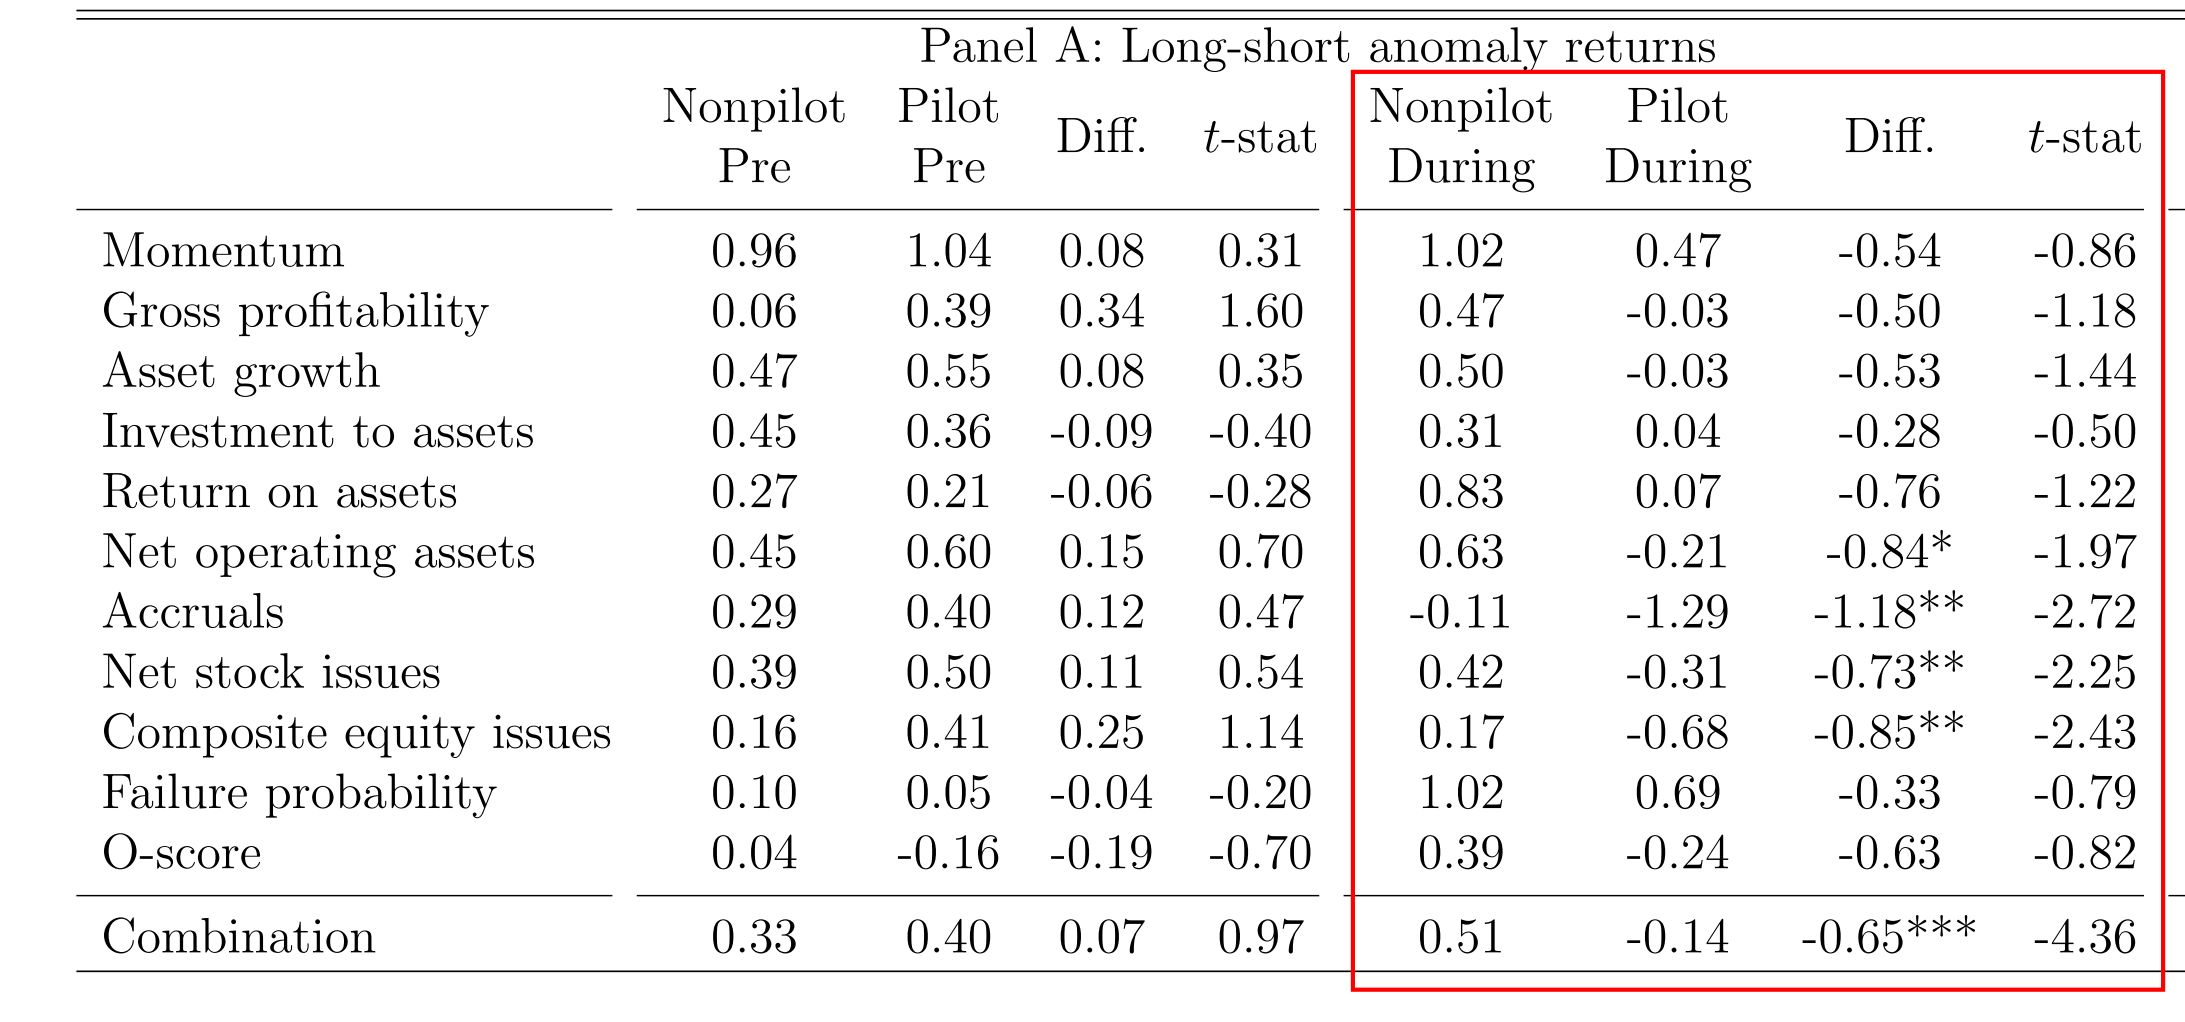
\includegraphics[scale=0.65,trim=1 1 1 1,clip]{figures/motivation_sho.jpg} 
	\label{tab:motivation_sho}%
\end{figure}

\vspace*{-1.2 cm}
{\tiny \qquad Source: \citet{Chu2016}}
	\begin{itemize}
		\item[$\rightarrow$] During the SHO Regulation the mispricing anomalies are not profitable in pilot stocks.
	\end{itemize}
\end{frame}  
%============================================================================
%============================================================================

\begin{frame}
\frametitle{SHO Experiment - Statistical Analysis}
\vspace*{-0.4cm}
{\scriptsize
		\begin{equation} \nonumber
 \beta^{MISP}_{l,t}(Pilot) - \beta^{MISP}_{l,t}(Control) = b_{0,l}  preD_t + b_{1,l}  announcementD_t + b_{2,l}  duringD_t + b_{3,l}  postD_t + \varepsilon_{l,t}
\end{equation}
}
\vspace*{-1cm}
\begin{table}[htbp]
  \centering
  \footnotesize
  	  \resizebox{0.7\textwidth}{!}{	 	
	 	% Table generated by Excel2LaTeX from sheet 'sho_experiment'
\begin{tabular}{lccc}
\toprule
        & (1)     & (2)     & (3) \\
        & Long Leg & Short Leg & Short - Long \\
\midrule
$preD$  & -0.0606 & -0.390** & -0.329 \\
        & (-0.90) & (-2.46) & (-1.60) \\
$announcementD$ & 0.407*** & -1.074*** & -1.480*** \\
        & (3.89)  & (-5.49) & (-5.00) \\
$duringD$ & 0.250** & -2.608*** & -2.858*** \\
        & (2.36)  & (-11.70) & (-11.18) \\
$postD$ & 0.729*** & 0.307   & -0.422 \\
        & (5.70)  & (1.66)  & (-1.63) \\
\midrule
$N$     & 52      & 52      & 52 \\
\bottomrule
\end{tabular}%

	\label{tab:sho_experiment}%
	}
\end{table}
\begin{itemize}
\item[$\rightarrow$] Difference in SR spreads is driven by the short side and is non-existent pre- and post-SHO. 
\end{itemize}

	\end{frame}
%============================================================================
	
%============================================================================
\begin{frame}
\frametitle{SHO Experiment - Graphical Analysis}
\vspace*{-0.3cm}
\begin{figure}[htbp]
\centering
	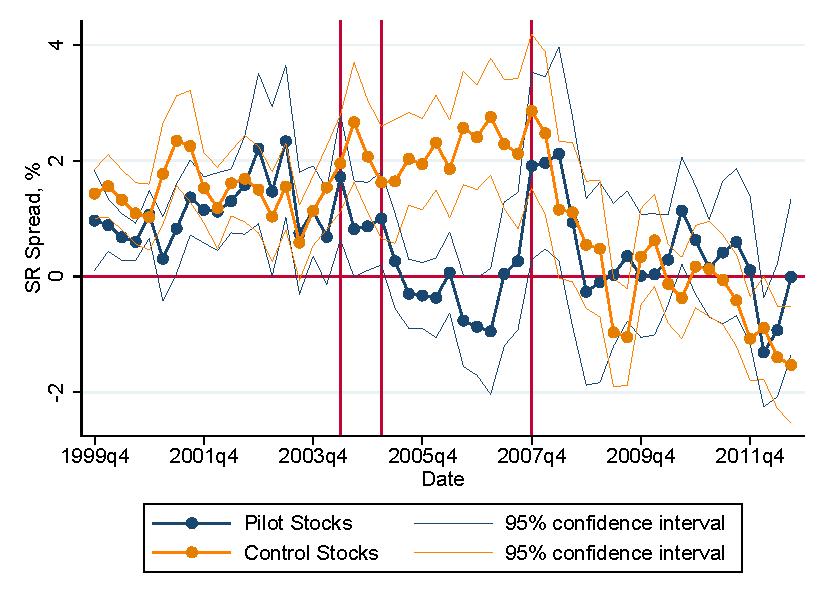
\includegraphics[scale=0.6,trim=4 4 4 4,clip]{figures/SHO_misp_graph.pdf} 
	\label{tab:SHO_misp_graph}%
\end{figure}
\begin{itemize}
\vspace*{-0.4cm}

\item[$\Rightarrow$] Short sellers cease exploiting the mispricing based anomaly in pilot stocks as a reaction to SHO Regulation. 
\end{itemize}
\end{frame}
%============================================================================

\begin{frame}
	\frametitle{SHO Experiment - Discussion}
\begin{itemize}
\item Lower abnormal returns due to decrease in limits to arbitrage drives short sellers away from the anomaly in pilot stocks. This result is consistent with the short sellers' ability to predict the effect of the regulation on the strategy returns.
\item Similarly to IVOL results, I do not observe the high-frequency short-sellers that arbitrage away the mispricing when it builds up.

\item[$\Rightarrow$] Short sellers profit from larger mispricing associated with higher limits to arbitrage.
 
%To analyze this process, in addition to high-frequency data, one needs the timing of mispricing shocks.
% \item  I observe the effect of low anomaly returns. In order to  
\end{itemize}
\end{frame}
%\item  Improved market efficiency is not driven by an increase in short positions. This finding contrasts to  \citet{Hanson2014} that predict lower anomaly returns to be driven by larger arbitrage capital, as proxied by SR spread. 
%\item Reasons of improved market efficiency:
%\begin{itemize}
%	\item Higher threat of short selling \citep[][]{Massa2015, Fang2016}
%	\item Improved efficiency of high-frequency trading \citep{Diether2009b}
%\end{itemize}
%\item Caveats: financial crisis, publication of anomalies, short sample period after 2007
%\item[$\Rightarrow$] In aggregate, my findings indicate less need in arbitrage capital for efficient markets due to decreasing limits-to-arbitrage.
%============================================================================

%============================================================================
\begin{frame}
\begin{center}
\Large Evolution of Arbitrage Capital and Profitability of Mispricing Strategy
\end{center}

\end{frame}
%============================================================================

%============================================================================
\begin{frame}
	\frametitle{Evolution of Arbitrage Capital}
	\framesubtitle{Spread in Short Interest Ratio}
	\begin{itemize}
		\item Does arbitrage activity decrease the profitability of mispricing strategy? Can short sellers time the strategy returns?   
		\item To answer this question, I contruct a proxy for arbitrage capital following  \citet{Hanson2014}. 		
		\item In each quarter $t$ I run the following pooled regression:
	\end{itemize}
\vspace*{0.3cm}
%{\scriptsize
		\begin{equation} \nonumber
			SR_{i,t} = \bm{\beta}^{MISP\prime}_{t}  \bm{D}^{MISP}_{it} +\bm{\beta}^{BM\prime}_{t}  \bm{D}^{BM}_{it}+\bm{\beta}^{Size\prime}_{t}  \bm{D}^{Size}_{it}   +\bm{\gamma}^\prime \bm{x}_{it} + \varepsilon_{i,t}
		\end{equation}
% +\bm{\beta}^{IVOL\prime}_{t}  \bm{D}^{IVOL}_{it}
%}
\begin{itemize}
\item \textbf{Spread in short interest ratio} of MISP strategy is defined as:
\end{itemize}
\vspace*{0.3cm}
\begin{equation} \nonumber
			S^{MISP}_{t} = \bm{\beta}^{MISP}_t[1] - \bm{\beta}^{MISP}_{t}[10]
		\end{equation}
\end{frame} 
%============================================================================	

%============================================================================
\begin{frame}
\frametitle{Evolution of Arbitrage Capital}
\framesubtitle{Short Interest Spread, Sentiment and Strategy Returns}
\vspace*{-0.3cm}
\begin{figure}[htbp]
\centering
	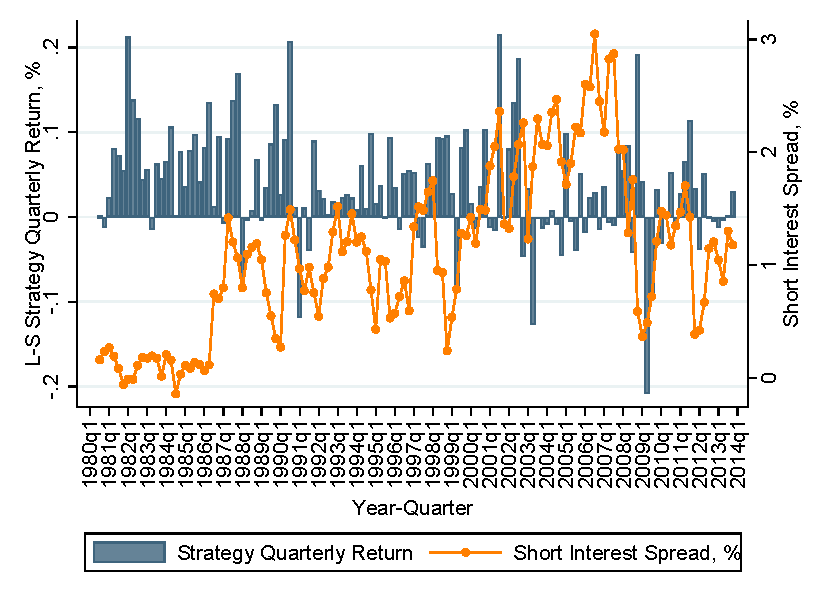
\includegraphics[scale=0.7,trim=4 4 4 4,clip]{figures/misp_evolution_profitability_yq_sentiment.pdf} 
	\label{tab:misp_evolution_profitability_yq_sentiment}%
\end{figure}
\begin{itemize}
\vspace*{-0.4cm}
\item[$\rightarrow$] Growth of strategy spread over time and a sharp decrease after 2007.
\end{itemize}
\end{frame}
%============================================================================
%============================================================================
\begin{frame}
\frametitle{Evolution of Arbitrage Capital}
\framesubtitle{Short Interest Spread, Sentiment and Strategy Returns}
\vspace*{-0.4cm}
		\begin{equation} \nonumber
Ret^{MISP}_{t} = \alpha+\beta_1  S^{MISP}_{t-1}  + \beta_2 Ret^{MISP}_{t-1} + \beta_3 Sent_{t-1} + \varepsilon_{t}
\end{equation}
\vspace*{-1cm}
\begin{table}[htbp]
  \centering
  \footnotesize
  	  \resizebox{\textwidth}{!}{	 	
	 	% Table generated by Excel2LaTeX from sheet 'misp_ret_breaks'
\begin{tabular}{l|ccc|cccc|}
\toprule
      & \multicolumn{1}{l}{1980-2013} & \multicolumn{1}{l}{1980-2002} & \multicolumn{1}{l|}{2002-2013} & \multicolumn{1}{l}{1980-2013} & \multicolumn{1}{l}{1980-2007} & \multicolumn{1}{l}{2008-2013} & \multicolumn{1}{l|}{2010-2013} \\
\midrule
$\_const$ & 0.0361*** & 0.0503*** & 0.00918 & 0.0353*** & 0.0513*** & -0.0769* & -0.0397 \\
      & (6.40) & (7.65) & (0.96) & (3.19) & (4.22) & (-1.96) & (-1.43) \\
$S_{misp}$ &       &       &       & -0.00880 & -0.0175** & 0.0930*** & 0.0586** \\
      &       &       &       & (-1.17) & (-2.32) & (2.95) & (2.52) \\
$Ret^{misp}_{t-1}$ &       &       &       & 0.00563 & -0.0379 & -0.0195 & -0.140 \\
      &       &       &       & (0.07) & (-0.39) & (-0.13) & (-0.85) \\
$Sent$ &       &       &       & 0.0320*** & 0.0248** & 0.0631 & 0.0427 \\
      &       &       &       & (3.52) & (2.58) & (1.52) & (1.37) \\
\midrule
$N$   & 134   & 89    & 45    & 133   & 110   & 23    & 15 \\
\bottomrule
\end{tabular}%

	\label{tab:misp_ret_breaks}%
	}
\end{table}
\begin{itemize}
\item[$\rightarrow$]The growth of arbitrage capital was until recently associated with lower returns of the mispricing-based strategy.
%\item[$\rightarrow$] Insignificant returns from mispricing strategy after 2002.
\item[$\rightarrow$] After 2007 short interest spread is positively associated with strategy profits, consistent with short-sellers' ability to time strategy returns.

\end{itemize}
	\end{frame}

%============================================================================
\begin{frame}
\frametitle{Supremum Wald Test}
\framesubtitle{Structural Break with Unknown Date}
\vspace*{-0.3cm}
\begin{itemize}
\vspace*{-0.4cm}
\item  I used supremum Wald test to determine whether the coefficients in a time-series regression vary over the periods defined by an unknown break date.
\item Full sample: 1980q3 - 2013q3
\item Coefficients included in the test: $\alpha$, $S^{MISP}_{t-1}$, $Ret^{MISP}_{t-1}$, $Sent_{t-1}$
\item Estimated break date: 2008q1
\end{itemize}
\begin{table}[htbp]
  \flushleft
  \centering
  	  \resizebox{0.35\textwidth}{!}{	 	
	 	% Table generated by Excel2LaTeX from sheet 'swald'
\begin{tabular}{lcc}
\toprule
Test  & Statistic & p-value \\
\midrule
swald  & 17.0959 & 0.0361 \\
\bottomrule
\end{tabular}%

	\label{tab:swald}%
	}
\end{table}
\begin{itemize}

\item[$\rightarrow$]Significant structural break in relationship in 2008.
\end{itemize}
\end{frame}
%============================================================================
%============================================================================
\begin{frame}
\frametitle{Supremum Wald Test}
\framesubtitle{Dynamics of Wald Test Statistic}

\begin{figure}[htbp]
\centering
	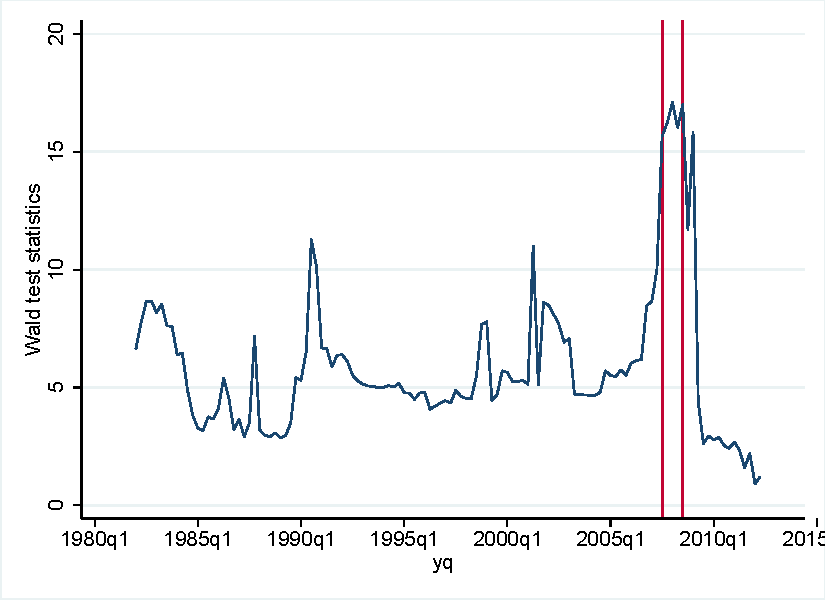
\includegraphics[scale=0.7,trim=1 1 1 1,clip]{figures/spread_structural_wald.pdf} 
	\label{tab:spread_structural_wald}%
\end{figure}
\begin{itemize}
\vspace*{-0.4cm}
\item[$\rightarrow$] The structural break is localized around the Quant Meltdown 2007 and the Financial Crisis 2008.
\end{itemize}
\end{frame}
%============================================================================	

%============================================================================

\begin{frame}[label=break_anomalies]
\frametitle{Structural Breaks - Anomalies}
\vspace*{-1cm}
\begin{table}[htbp]
  \centering
  \footnotesize
  	  \resizebox{\textwidth}{!}{	 	
	 	% Table generated by Excel2LaTeX from sheet 'break_anomalies'
\begin{tabular}{lccccccc}
\toprule
\multicolumn{1}{c}{Anomaly} & Published & Return Break Date & $\Delta$ Ret & t-stat & Relationship Break Date & $\Delta S^{MISP}$  & t-stat \\
\midrule
MISP  & 2012  & 2002  & -0.035 & -4.05 & 2008  & 0.075 & 2.84 \\
NI    & 1991  & 1987  & -0.022 & -3.89 & 2002  & 0.023 & 1.81 \\
CEI   & 2006  & 1998  & 0.015 & 1.70  & 2008  & 0.047 & 2.66 \\
ACC   & 1996  & 2000  & -0.017 & -2.50 & 2008  & 0.025 & 0.88 \\
NOA   & 2004  & 1999  & -0.020 & -2.20 & 1998  & 0.003 & 0.15 \\
AG    & 2008  & 2000  & -0.013 & -1.71 & 1986  & 0.009 & 0.24 \\
ITA   & 2004  & 1999  & -0.021 & -2.56 & 2008  & 0.009 & 0.38 \\
FD    & 2008  & 1986  & -0.048 & -3.16 & 2007  & 0.029 & 1.90 \\
OS    & 1980  & 1985  & -0.033 & -3.20 & 1997  & 0.023 & 1.80 \\
MOM   & 1993  & 2008  & -0.062 & -2.63 & 2001  & 0.010 & 0.53 \\
GPP   & 2010  & 1990  & -0.028 & -2.97 & 1998  & 0.019 & 1.17 \\
ROA   & 2006  & 1986  & -0.052 & -4.31 & 1999  & 0.022 & 1.55 \\
\bottomrule
\end{tabular}%

	\label{tab:break_anomalies}%
	}
\end{table}
\begin{itemize}
\item[$\rightarrow$] Structural break is driven by multiple anomalies.
\end{itemize}
\hfill \hyperlink{aum_spread_correlate}{\beamerbutton{AUM Correlation Break Date}}
	\end{frame}
%============================================================================

%============================================================================

\begin{frame}
\frametitle{Do Short Sellers Profit from the Mispricing Timing?}

\begin{itemize}
\item Assume $S^{MISP}_y$ is the average exposure to $MISP$.
\item $S^{MISP}_q$ is the most recent exposure to $MISP$.
%\item $\frac{S^{MISP}_q}{S^{MISP}_y}$ is the share of average capital employed recently.
\item  $Ret^{Misp}\frac{S^{MISP}_q}{S^{MISP}_y} - Ret^{Misp} $ is the difference in returns of the most recent capital employed and the average capital employed
\item This measure proxies for profits from short sellers' timing skill.
% =Ret^{Misp}\frac{(S^{MISP}_q-S^{MISP}_y)}{S^{MISP}_y}
\end{itemize}

\begin{table}[htbp]
  \centering
  \footnotesize
  	  \resizebox{0.65\textwidth}{!}{	 	
	 	% Table generated by Excel2LaTeX from sheet 'misp_timing'
\begin{tabular}{ccc|c}
\toprule
      & (1)   & (2)   & (3) \\
      & \multicolumn{1}{l}{$Ret^{MISP}$} & \multicolumn{1}{l|}{$Ret^{MISP}\frac{S^{MISP}_{Q}}{S^{MISP}_{Y}}$} & \multicolumn{1}{l}{$Diff = (2) - (1)$} \\
\midrule
1980-2013 & 0.0361*** & 0.0419*** & 0.00581 \\
      & (4.79) & (4.20) & (1.41) \\
      &       &       &  \\
1980-2008 & 0.0414*** & 0.0468*** & 0.00539 \\
      & (5.57) & (4.30) & (1.09) \\
      &       &       &  \\
2008-2013 & 0.00924 & 0.0172*** & 0.00795* \\
      & (1.37) & (3.51) & (1.78) \\
\bottomrule
\end{tabular}%

	\label{tab:misp_timing}%
	}
\end{table}
\begin{itemize}
\item[$\rightarrow$] Short-sellers time the mispricing after 2008 well.
\end{itemize}
	\end{frame}
%============================================================================


%============================================================================
\begin{frame}

\frametitle{Evolution of Arbitrage Capital}
\framesubtitle{Discussion}
\begin{itemize}
\item Rise of arbitrage capital in 2000s is associated with a decrease in anomaly profits.
\item Structural break in the behaviour after the Quant Meltdown and the Financial Crisis (2007-2008).
\item Short sellers time mispricing after 2008 well.
\item[$\Rightarrow$] Short sellers consistently profit from the mispricing.  

\end{itemize}
\end{frame}
%============================================================================
%============================================================================
%
%
%\begin{frame}
%	\frametitle{Possible Extensions}
%\begin{itemize}
%\item High-frequency data on short positions could be used to test whether low anomaly returns and low SR spread for pilot stocks during the SHO experiment are caused by high-frequency short-sellers \citep{Diether2009b}.
%\item Test whether short-sellers exploit beta anomaly and whether this trading activity can be explained by relation to IVOL anomaly \citep{Liu2016}.
%
%\end{itemize}
%\end{frame}

%============================================================================


	\section{Conclusion}
	\begin{frame}
		\frametitle{Conclusion}
		\begin{itemize}
		\item This study shows that short sellers are smart anomaly traders as they:
		\begin{itemize}
		\item Consistently exploit mispricing-based anomaly.
		\item Profit from stocks with larger mispricing due to higher limits to arbitrage and higher sentiment.
		\item Posses mispricing returns timing ability.
		\end{itemize}
		\item Short-sellers contribute to market efficiency by eliminating anomalies \citep{Hanson2014, Akbas2015, Mclean2016}.
		\item  Supporting evidences in favor of existing theories of limits to arbitrage \citep[][]{Shleifer1997, Pontiff2006, Stambaugh2015} and sentiment-driven mispricing \citep{Baker2006}.
		\end{itemize}
	\end{frame}  
%============================================================================
%============================================================================	
%\begin{frame}
%	\frametitle{Title}
%	{\scriptsize
%		\begin{equation} \nonumber
%			Ret_{i,t} = \alpha_t+\beta_1  SUSIR_{i,t-1} +   \sum_{k=2}^5 \beta_k M_{Quintile=k,i,t-1} + \sum_{k=2}^5 \gamma_k SUSIR_{i,t-1} \times  M_{Quintile=k,i,t-1}  + \mathbf{x'_{i}} \mathbf{b}+ \varepsilon_{i,t}
%		\end{equation}
%	}
%	\begin{table}[htbp]
%	  \centering
%	  \footnotesize
%	  \resizebox{0.7\textwidth}{!}{
%			% Table generated by Excel2LaTeX from sheet 'limits_to_arbitrage_short'
\begin{tabular}{lccc}
\toprule
        & $M = HLSPREAD$ & $M = IVOLA$ & $M = RIO$ \\
        & (1)     & (2)     & (3) \\
        & $Ret_{i,t}$ & $Ret_{i,t}$ & $Ret_{i,t}$ \\
\midrule
$SUSIR$ & -0.0816** & -0.0352 & -0.0893*** \\
        & (-2.49) & (-1.06) & (-2.84) \\
$SUSIR \times M_{Quintile=2}$ & 0.0339  & -0.0618* & -0.0164 \\
        & (0.87)  & (-1.74) & (-0.35) \\
$SUSIR \times  M_{Quintile=3}$ & -0.0287 & -0.0837* & -0.0267 \\
        & (-0.57) & (-1.79) & (-0.58) \\
$SUSIR \times  M_{Quintile=4}$ & -0.0545 & -0.0928* & -0.0687 \\
        & (-1.16) & (-1.87) & (-1.35) \\
$SUSIR \times  M_{Quintile=5}$ & -0.154*** & -0.141** & -0.0209 \\
        & (-3.07) & (-2.38) & (-0.32) \\
\midrule
$Controls$ & Yes     & Yes     & Yes \\
$R^2$   & 0.0684  & 0.0719  & 0.0689 \\
$N$     & 577088  & 576894  & 575995 \\
\bottomrule
\end{tabular}%

%			\label{tab:limits_to_arbitrage}%
%		}
%	\end{table}
%
%	\begin{figure}[htbp]
%		\centering
%		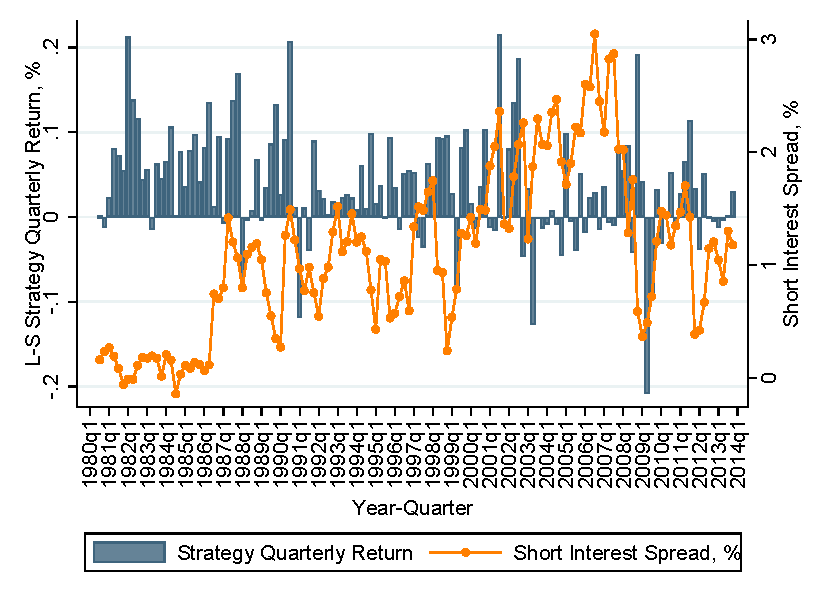
\includegraphics[scale=0.7,trim=4 4 4 4,clip]{figures/misp_evolution_profitability_yq_sentiment.pdf} 
%		\label{tab:misp_evolution_profitability_yq_sentiment}%
%	\end{figure}
%
%	\begin{itemize}
%		\item 		
%	\end{itemize}
%\end{frame}  
%============================================================================
	\section{Appendix}
	\begin{frame}
		\centering
		\frametitle{}
	\huge{Appendix}
	\end{frame}



%============================================================================

\begin{frame}
	\frametitle{Descriptive Statistics}
\begin{table}[htbp]
  \centering
  \footnotesize
	  \resizebox{0.7\textwidth}{!}{
	% Table generated by Excel2LaTeX from sheet 'summary'
\begin{tabular}{lccccccc}
\hline
\hline
\multicolumn{8}{l}{Panel A: Summary Statistics} \bigstrut\\
\hline
        &         &         & \multicolumn{5}{c}{Percentiles} \bigstrut\\
\cline{4-8}\multicolumn{1}{c}{Variable} & Mean    & SD      & 1st     & 10th    & Median  & 90th    & 99th \bigstrut\\
\hline
$SUSIR$ & 0.334   & 0.403   & -0.718  & -0.159  & 0.348   & 0.800   & 1.555 \bigstrut[t]\\
$SR$    & 0.027   & 0.023   & 0.003   & 0.005   & 0.018   & 0.060   & 0.094 \\
$DTC$   & 5.479   & 2.142   & 1.467   & 2.095   & 5.787   & 7.959   & 10.046 \\
$SR_{IO}$ & 0.058   & 0.024   & 0.023   & 0.032   & 0.050   & 0.091   & 0.129 \\
$MBETA$ & 1.056   & 0.063   & 0.865   & 0.990   & 1.048   & 1.143   & 1.163 \\
$SIZE$  & 3939.353 & 2230.917 & 896.804 & 1153.332 & 3571.290 & 6905.367 & 8159.658 \\
$BM$    & 0.670   & 0.123   & 0.449   & 0.504   & 0.665   & 0.840   & 0.965 \\
$RET\_RV$ & 0.012   & 0.050   & -0.117  & -0.046  & 0.017   & 0.070   & 0.120 \\
$RET\_MOM$ & 0.185   & 0.208   & -0.283  & -0.067  & 0.178   & 0.413   & 0.851 \\
$INV$   & 0.161   & 0.041   & 0.067   & 0.108   & 0.161   & 0.215   & 0.236 \\
$ROA$   & 0.053   & 0.016   & 0.009   & 0.032   & 0.054   & 0.066   & 0.091 \\
$MISP$  & 48.879  & 1.224   & 45.616  & 47.089  & 49.145  & 50.092  & 51.506 \\
$IVOLA$ & 0.019   & 0.004   & 0.014   & 0.015   & 0.018   & 0.024   & 0.032 \\
$HLSPREAD$ & 0.007   & 0.002   & 0.005   & 0.006   & 0.007   & 0.010   & 0.017 \\
$IO$    & 0.514   & 0.149   & 0.268   & 0.303   & 0.488   & 0.730   & 0.761 \bigstrut[b]\\
\hline
\end{tabular}%

	\label{tab:summary}%
	}
\end{table}
	\end{frame}
%============================================================================

%============================================================================
\begin{frame}
\frametitle{Abnormal Short Interest Over Size Deciles}

\begin{figure}[htbp]
	\centering
	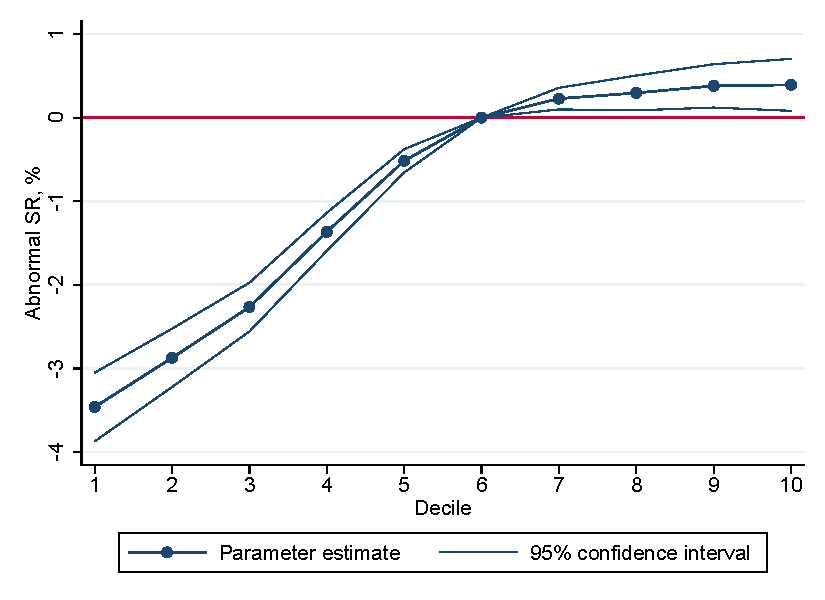
\includegraphics[scale=0.7,trim=4 4 4 4,clip]{figures/size_sr_by_decile_fe.pdf} 
	\label{tab:size_sr_by_decile_fe}%
\end{figure}
		\vspace*{-0.4cm}

\end{frame}
%============================================================================
\begin{frame}

\frametitle{Abnormal Short Interest Over Book-To-Market Deciles}


\begin{figure}[htbp]
	\centering
	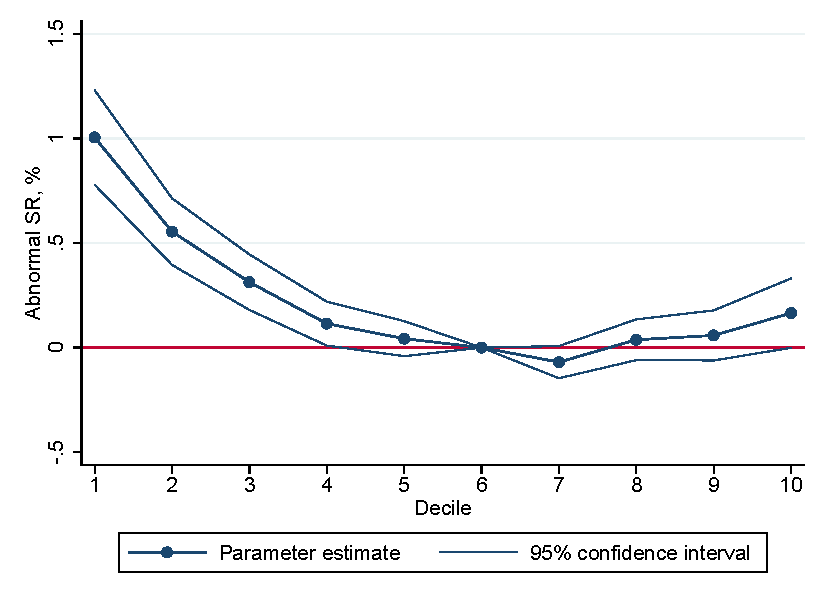
\includegraphics[scale=0.7,trim=4 4 4 4,clip]{figures/bm_sr_by_decile_fe.pdf} 
	\label{tab:bm_sr_by_decile_fe}%
\end{figure}
		\vspace*{-0.4cm}

\end{frame}
%============================================================================
%============================================================================

\begin{frame}
\frametitle{Other variables}

\vspace*{-0.1cm}
\begin{table}[htbp]
  \centering
  \footnotesize
  	  \resizebox{0.4\textwidth}{!}{	 	
	 	% Table generated by Excel2LaTeX from sheet 'sr_by_decile_short'
\begin{tabular}{llc}
\toprule
        & \multicolumn{1}{c}{(1)} & (2) \\
        & \multicolumn{1}{c}{SR} & SR \\
\midrule
$Turn$  & \multicolumn{1}{c}{13.29***} & 11.25*** \\
        & \multicolumn{1}{c}{(11.82)} & (12.40) \\
$IO$    & \multicolumn{1}{c}{3.059***} & 6.242*** \\
        & \multicolumn{1}{c}{(12.11)} & (18.10) \\
$IVOL$  & \multicolumn{1}{c}{-2.219} & -2.458 \\
        & \multicolumn{1}{c}{(-0.46)} & (-0.95) \\
$D\_convert$ & \multicolumn{1}{c}{0.641***} & 0.758*** \\
        & \multicolumn{1}{c}{(7.55)} & (9.52) \\
$D\_sp500$ & \multicolumn{1}{c}{-0.463***} & -0.520*** \\
        & \multicolumn{1}{c}{(-5.21)} & (-4.19) \\
$D\_nasdaq$ & \multicolumn{1}{c}{0.920***} & 0.490 \\
        & \multicolumn{1}{c}{(6.11)} & (1.37) \\
$D\_nyse$ & \multicolumn{1}{c}{0.365***} & 0.362** \\
        & \multicolumn{1}{c}{(3.12)} & (2.08) \\
$Illiq$ & \multicolumn{1}{c}{-0.0615**} & -0.0321* \\
        & \multicolumn{1}{c}{(-2.11)} & (-1.86) \\
$Acoverage$ & \multicolumn{1}{c}{0.0305***} & 0.0449*** \\
        & \multicolumn{1}{c}{(4.12)} & (7.76) \\
\midrule
Misp Decile Dummies & \multicolumn{1}{c}{Yes} & Yes \\
SIZE Decile Dummies & \multicolumn{1}{c}{Yes} & Yes \\
BM Decile Dummies & \multicolumn{1}{c}{Yes} & Yes \\
Time Fixed Effects & \multicolumn{1}{c}{Yes} & Yes \\
Stock Fixed Effects & \multicolumn{1}{c}{No} & Yes \\
N       & 575371  & 575279 \\
R-sq    & 0.503   & 0.705 \\
\bottomrule
\end{tabular}%

	\label{tab:sr_by_decile_short}%
	}
\end{table}

\begin{itemize}
\item[$\rightarrow$] Stock fixed effect account for around 20\% of SR variation.
\end{itemize}
	\end{frame}

%============================================================================
%============================================================================	
\begin{frame}
		\frametitle{Entering Extreme Deciles - High vs. Low IVOL}
		\framesubtitle{Methodology}	
	\begin{itemize}
		\item To test how short interest evolves around stock’s entering the extreme decile:
	\end{itemize}
{\scriptsize
		\begin{equation}		 \nonumber
		\begin{split}
			SR_{i,t} &= [h^{-24} D^{-24}_{it}(MISP) + \ldots +h^{0} D^0_{it}(MISP) + \ldots + h^{+24} D^{+24}_{it}(MISP)]\times 1\{ ivolH =1 \}+  \\
			& + [l^{-24} D^{-24}_{it}(MISP) + \ldots +l^{0} D^0_{it}(MISP) + \ldots + l^{+24} D^{+24}_{it}(MISP)]\times 1\{ ivolL =1 \}+ \\
			&+\bm{\beta}^{IVOL\prime}  \bm{D}^{IVOL}_{it} + \bm{\beta}^{BM\prime}  \bm{D}^{BM}_{it}+\bm{\beta}^{Size\prime}  \bm{D}^{Size}_{it}  +\bm{\gamma}^\prime \bm{x}_{it} + Time_t +  \varepsilon_{i,t}
		\end{split}
		\end{equation}
}
\begin{itemize}
\item[]
\begin{itemize}
\item $D^0_{it}(MISP)$ - dummy that is equal to one for all months when the stock is in the mispricing decile 1.
\item $D^{-24}_{it}(MISP)$ - dummy that is equal to one if the stock enters the mispricing decile 1 in 24 months from t.
\item $D^{+24}_{it}(MISP)$ - dummy that is equal to one 24 months after the stock enters the mispricing decile 1.

\end{itemize}
\end{itemize}
\end{frame}  




%============================================================================

%============================================================================

\begin{frame}[label=ivol_dynamics]
		\frametitle{Short Interest and IVOL - Entering Extreme Deciles\hfill \hyperlink{ivol_results}{\beamerbutton{back}}}
		\vspace*{-0.2cm}
{\scriptsize Extreme Overpriced Decile (upper graph) and Extreme Underpriced Decile (lower graph) }
\vspace*{-0.8cm}
		\begin{columns}
 \begin{column}{.5\textwidth}         
\begin{figure}[htbp]
	 \centering
	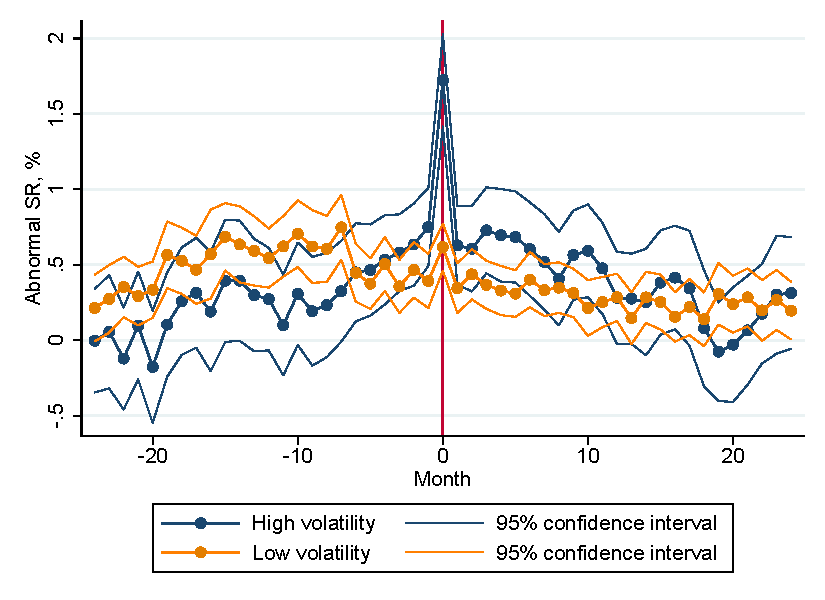
\includegraphics[scale=0.431]{figures/misp_event_time_sr_dec1.pdf} 
	% \caption[]{\textbf{\\Cumulative Logarithmic Raw Returns}\\
    % \footnotesize{Plotted are the monthly cumulative sum of log raw returns for equal-weighted and value-weighted $SUSIR$ long-short strategy over the period from March 1980 to December 2013.}}
\end{figure}
\vspace*{-2.1cm}
\begin{figure}[htbp]
	 \centering
	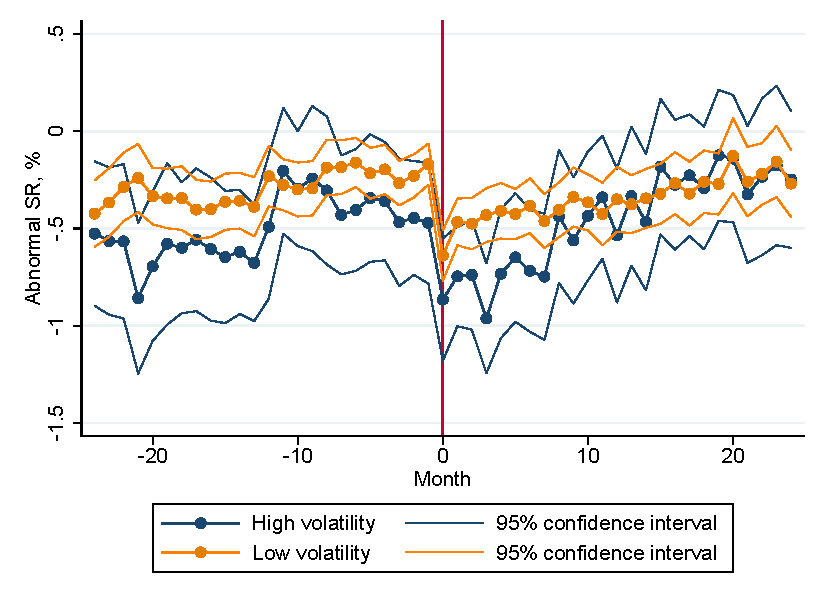
\includegraphics[scale=0.431]{figures/misp_event_time_sr_dec10.pdf} \\
\end{figure}
\end{column}

\begin{column}{.5\textwidth}
\vskip1ex
\begin{itemize}
\justifying
\item High and low volatility are top 30\% and bottom 30\% IVOL stocks in the recent month, correspondingly.
\item Strong change in short interest upon entering extreme overpriced decile for high-IVOL stocks
\item Much weaker reaction for low-IVOL stocks.
\item  Similar but weaker pattern upon entering extreme underpriced decile.
\item[$\Rightarrow$] Intended changes in short position.
% (to maximize returns from exploiting mispricing)
\end{itemize}
\end{column}
\begin{column}{.01\textwidth}
\end{column}

   \end{columns}

\end{frame}
%============================================================================
%============================================================================

\begin{frame}[label=aum_spread_correlate]
\frametitle{Break Date in Correlation between SR Spread and AUM}
\vspace*{-0.2cm}

\begin{itemize}
\item I correlate the SR spread with the AUM of hedge funds.
\item $AUM^{MN}_y$ is one year moving average AUM of market neutral equity hedge funds from Barclay Hedge.
\item $S^{MISP}_y$ is the one year moving average spread in SR.
\item Estimated correlation:
\end{itemize}

\vspace*{-0.2cm}
\begin{table}[htbp]
  \centering
  \footnotesize
  	  \resizebox{0.6\textwidth}{!}{	 	
	 	% Table generated by Excel2LaTeX from sheet 'aum_spread_correlate'
\begin{tabular}{lccc}
\toprule
      & \multicolumn{1}{l}{2000-2013} & \multicolumn{1}{l}{2000-2008} & \multicolumn{1}{l}{2008-2013} \\
      & $S^{MISP}_y$ & $S^{MISP}_y$ & $S^{MISP}_y$ \\
\midrule
$\_cons$ & 1.552*** & 1.667*** & 1.057*** \\
      & (6.82) & (14.72) & (4.26) \\
$AUM^{MN}_y$ & 0.00430 & 0.0175*** & 0.00127 \\
      & (0.56) & (3.84) & (0.16) \\
\midrule
$Correlation$ & 0.0769 & 0.711 & 0.0214 \\
N     & 55    & 31    & 24 \\
\bottomrule
\end{tabular}%

	\label{tab:aum_spread_correlate}%
	}
\end{table}
\begin{itemize}
\item[$\rightarrow$] Same date of structural break in correlation (Estimated date: 2008q2) %of $S^{MISP}$ with $AUM^{MN}$.
\item[$\rightarrow$] Highly correlated growth of $S^{MISP}$ and AUM before 2008 but weak relation after 2008. Consistent with short sellers' less reliance on known mispricing anomalies over time \citep{Wu2014}. \hfill \hyperlink{break_anomalies}{\beamerbutton{Back}} 
\end{itemize}
	\end{frame}
%============================================================================	
	\end{document}
